\documentclass[]{article}
\usepackage[czech]{babel}
\usepackage[utf8]{inputenc}
\usepackage{float}
\usepackage{graphicx}


\begin{document}

\title{Kapitola 2: Techniky modelování podnikových procesů}
\author{Bc. Štěpán Heller}
\date{\today}
\maketitle

\section{Procesní model a důvody pro jeho tvorbu}
Ať už člověk vytváří jakýkoliv model, jeho cílem je zachytit nějaký jev, který je potřeba kvůli své komplexnosti zobrazit zjednodušenou vizuální formou, která bude pochopitelná i pro jiné lidi než je sám tvůrce modelu. Umět jev zachytit ve formě modelu je jedním z prvních kroků na cestě k tomu tento jev upravovat.

Přeneseno do světa podnikových procesů je to velmi podobné. Jedním z hlavních důvodů, proč organizace přistupují k práci s BPM je potřeba procesy upravovat a zejména optimalizovat. Aby to bylo možné, je potřeba nejdřív stanovit metriky a tyto metriky být pak schopen měřit. Základem pro všechny tyto kroky je ale korektní procesní model, který proces věrně popisuje.

\subsection{Definice procesního modelu}
Základní definice procesního modelu podle 
\begin{quote}
Procesní model je konceptualizací podnikového procesu v organizaci.
\footnote{Process model is a conceptualization of the (business) process in an enterprise. \cite{Dietz2006}}
\end{quote}
Čtenářsky přístupnější definici pak nabízí \cite{Recker2009}
\begin{quote}
Procesní model popisuje, většinou grafickou formou aktivity, události, jejich pořadí a propojení, které utváří podnikový proces.
\footnote{Process model describe, typically in a graphical way, the activities, events and control flow logic that constitues a business process.}
\end{quote}

\section{Základní techniky}
V této sekci si popíšeme populární techniky pro tvorbu procesních modelů.
\subsection{Vývojový diagram (flowchart)}
Vývojový diagram je pravděpodobně nejpopulárnější technikou pro modelování podnikových procesů. Vděčí za to zejména své jednoduchosti, dostupnosti mnoha nástrojů, které tuto techniku podporují a také její velké srozumitelnosti, která jí činá velmi snadno uchopitelnou i pro uživatele v organizaci, kteří nejsou příliš obeznámeni s problematikou modelování podnikových procesů.

\subsubsection{Základní pravidla}
Vývojové diagramy se skládají z několika málo základních symbolů. Tyto symboly se nazývají: \cite{Chytil2005}

\begin{itemize}
\item Startovací a ukončovací symboly – používají se pro vyznačení začátku a konce procesu
\item Šipky – zobrazují tzv. \uv{řídící tok}, tedy přechod v čase mezi jednotlivými symboly
\item Dílčí kroky procesu – jsou reprezantovány obdelníkem.
\item Podprogramy – zobrazeny obdelníkem se svislými čarami po stranách. Používají se pro zobrazení skupiny kroků procesu pomocí jediného symbolu.
\item Vstupy a výstupy – zobrazují tok informací směrem dovnitř i vně procesu, Pro jejich reprezentaci se používají lichoběžníky respektive rovnoběžníky.
\item Podmíněný cyklus – zobrazuje událost opakující dokud je splněna jasně definovaná podmínka. Zobrazuje se pomocí šestiúhelníku.
\item Podmíněný výraz – kosočtvercem je symbolizováno rozhodnutí a určuje tedy místo, kde dochází k větvení procesu.
\item Spojovací symbol – inverzním symbolem ke kosočtverci je ve vývojovém diagramu kruh, který se používá ke spojení více toků do jednoho.
\end{itemize}

\begin{figure}[H]\centering %todo překreslit obrázek%
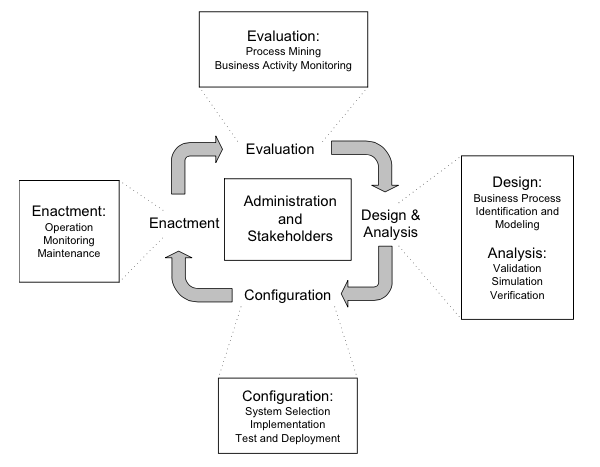
\includegraphics[width=1.0\textwidth]{obrazky/processLifecycle}
\caption{Business Process Lifecycle \cite{Weske2007}}
\label{fig:BusinessProcessLifecycle}
\end{figure}

\subsubsection{Výhody a nevýhody}
Nespornou výhodou vývojových diagramů je právě jejich přístupnost pro uživatele a velmi strmá křivka učení, což dělá z této techniky první volbu pro případy, kdy je potřeba velmi rychle vymodelovat nějaký proces a organizace nemá zavedeny sofistikovanější metody BPM. Vývojové diagramy umožňují efektivnější komunikaci o problému v rámci týmu. 

Největší přednost vývojových diagramů je zároveň jejich největší slabinou. Právě přílišná jednoduchost této techniky dělá z modelování komplexnějších procesů poměrně komplikovanou a nepřehlednou záležitostí. Ve vývojových diagramech je také složitější modelovat některé jevy, jako například tzv. \uv{unhappy paths} a další nestandardní události, která však v životě procesů nastávají poměrně běžně. U vývojových diagramů je také obtížné dělat změny, protože to často vyžaduje kompletní překreslení celého diagramu.

\subsubsection{Použití}
Vývojové diagramy mají mnoho využití. Hodí se například pro komunikaci mezi organizací a jejími externími zákazníky, protože se dá předpokládat, že se s vývojovými diagrami už v minulosti setkali a budou jim tedy rozumět. Vhodné je také použít vývojový diagram v dokumentaci k softwaru nebo jinému systému, kterou budou číst různorodé skupiny uživatelů.

\subsection{BPMN}
S trochou nadsázky by se dalo říct, že BPMN je vlastně rozšířením vývojového diagramu. Je určitě pravdou, že se BPMN touto jednoduchou technikou v mnohém inspirovalo a na jejích základech postavilo notaci, která umožňuje poměrně jednoduše modelovat i komplexní podnikové procesy a zároveň si stále uchovává dobrou srozumitelnost pro uživatele.

\subsection{BPEL}
\subsection{UML}
\subsection{Petriho sítě}
\subsection{DEMO}
\section{Srovnání technik}

\nocite{*}
\bibliographystyle{plain}
\bibliography{Bibliography}

\end{document}